\section{Human-System Interaction Ergonomics}

The following section focuses on the selected topics of Human-System Interaction Ergonomics: Accessibility, Usability, and \gls{ux}.
The selected topics are explored in relation to computer software and, where possible, web services specifically.
After introducing the concepts, this section focuses on non-obvious benefits and delves into the implementation and evaluation strategies.
This section strives to introduce the topics and then dive deeper into pragmatic information relevant to this thesis.

\subsection{Definition and Distinction}
\label{Literature-HSIE-Definition}

Considering there are incompatible definitions for Accessibility provided by \gls{iso} \parencite{Wegge_Zimmermann_2007}, the specific definition chosen for this thesis describes Accessibility as the "extent to which [a service] can be used by people from a population with the widest range of user needs, characteristics and capabilities to achieve identified goals [...]" \parencite{ISO_9241-11:2018}.
\textcite{ISO_10779:2020} adds that Accessibility includes but does not apply exclusively to formally disabled people.
That means Accessibility is concerned with the basic ability to utilise the software by the widest possible range of users, including disabled users \parencite{Wegge_Zimmermann_2007}.
Similar concepts include "design for all", "inclusive design", or "universal design" \parencite[p. 1210]{Juergen_et_all_2020} with a viewpoint of designing services for all types of people, including the disabled.
\textcite{Wegge_Zimmermann_2007} point to existing confusion between the terms Accessibility and Usability.
Although \textcite{Wegge_Zimmermann_2007} admit these terms are related and have potential overlap, \textcite{Wegge_Zimmermann_2007} stress the importance of their distinction.
Importantly, \gls{ict} is one of the fields where Accessibility, depending on the country and sector, is mandated by the law \parencite{Wegge_Zimmermann_2007, Juergen_et_all_2020}.
For example, public sector services within \gls{eu} have to meet accessibility standards outlined in the Web Accessibility Directive, and there is an ongoing effort to extend this to the private sector \parencite{EU_Web_Accessibility}.

Usability, on the other hand, is defined by \textcite{ISO_9241-11:2018} as the "extent to which [a service] can be used by specified users to achieve specified goals with effectiveness, efficiency and satisfaction [...]".
As \textcite{Wegge_Zimmermann_2007} hint, compared to Accessibility, Usability deals with the success - "effectiveness, efficiency and satisfaction" \parencite{ISO_9241-11:2018} - of software interactions which is hard to mandate the way Accessibility is.
Therefore, there are few relevant laws and Usability is usually considered more as a competitive advantage that authors are trying to capitalise on \parencite{Wegge_Zimmermann_2007}.

Similarly to confusion between Accessibility and Usability, researchers point to issues with the distinction between Usability and User Experience \parencite{Darin_et_all_2019, Juergen_et_all_2020}.
There are multiple views on the definition of \gls{ux} and a great amount of disagreement on the topic \parencite{Juergen_et_all_2020}.
\textcite{ISO_9241-11:2018} defines \gls{ux} as "user’s perceptions and responses that result from the use and/or anticipated use of [a service]".
Compared to the sole satisfaction that was mentioned to be a part of Usability and \textcite{Darin_et_all_2019} argue is incorrectly used as, and often only, \gls{ux} measurement, \gls{ux} deals with "users’ emotions, beliefs, preferences, perceptions, comfort, behaviours, and accomplishments" \parencite{ISO_9241-11:2018}.
Additionally, \gls{ux} is concerned with a broader timeline - the time spent performing the task \emph{and} the time before and after that \parencite{Juergen_et_all_2020,ISO_9241-11:2018}.
Considering the definition by \textcite{ISO_9241-11:2018} and in partial disagreement with \textcite{Darin_et_all_2019}, we can look at \gls{ux} as a concept that overlaps with Usability or a whole complex superset of Usability \parencite{Juergen_et_all_2020}.

In short, for the purposes of this thesis, Accessibility is the basic ability to use the software regardless of the user's various limitations, Usability is the extent to which it can be used to achieve delineated goals successfully, and \gls{ux} is a more complex extension also concerned with impressions both during and outside of the use of the software.
The following subsections always refer to these ideas as Accessibility, Usability, and \gls{ux}, even if cited literature refers to them differently.

\begin{figure}[H]
    \centering
    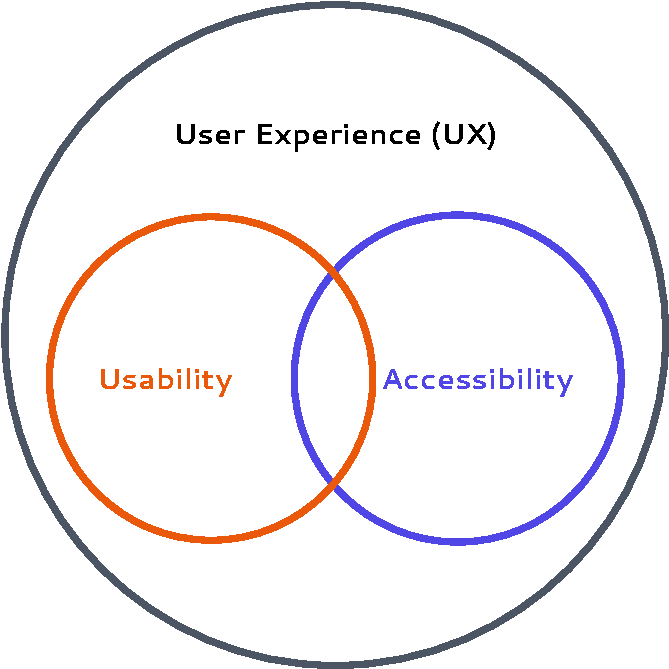
\includegraphics[height=8cm, keepaspectratio]{Accessibility_Usability_UX_Diagram}
    \caption{Relation between Accessibility, Usability, and \gls{ux}.}
    \label{fig:hsie-relations}
\end{figure}

\subsection{Benefits}
\label{Literature-HSIE-Benefits}

\textcite{Juergen_et_all_2020} point to their earlier research results that indicate implementing Accessibility on the web could provide benefits to users other than the usual primary target of Accessibility enhancements - disabled users \parencite{Schmutz_Sonderegger_Sauer_2016, Schmutz_Sonderegger_Sauer_2017, Schmutz_Sonderegger_Sauer_2018}.
This notion is seconded by \textcite{Vanderheiden_2000}, who mentions that others in similar challenging situations can benefit from Accessibility as well.
\textcite{Edyburn_2010} provides terminology identifying these two groups of users: primary and secondary beneficiaries. Specifically in the educational setting, \textcite{Edyburn_2021} mentions that Accessibility can improve the ability to use the software for both primary beneficiaries - disabled students - and secondary beneficiaries - all other students.

Examples of secondary beneficiaries concerning the web are mentioned by \textcite{WAI_Intro}:

\begin{itemize}
    \item people using different devices with smaller screens or "different input modes" \parencite{WAI_Intro},
    \item people challenged by limitations introduced by ageing,
    \item temporarily limited people - e.g. by a "broken arm or lost glasses [...or a] bright sunlight" \parencite{WAI_Intro}, or conditions that do not allow audio playback,
    \item and people limited by their internet connection - i.e. latency or bandwidth.
\end{itemize}

However, \textcite{Juergen_et_all_2020} also mention that benefits from some specific concepts could be limited. For example, "using easy language" \parencite[p. 1210]{Juergen_et_all_2020} was shown to have limited benefits and considerable disadvantages like decreased enjoyment and higher required time to consume the content \parencite{Schmutz_Sonderegger_Sauer_2019}.

As for the Usability and \gls{ux} benefits, as was already mentioned in \autoref{Literature-HSIE-Definition}, these can be used as a competitive advantage \parencite{Wegge_Zimmermann_2007}, or, more specifically, to improve some metric like conversion rate, traffic numbers, user performance, or usage of key features \parencite{Nielsen_2008}.
Surveys summarised by \textcite{Nielsen_2008} indicate a high, double-digit \gls{roi} even though this number is declining year on year, presumably due to the ever-improving starting state.

\subsection{Implementation}
\label{Literature-HSIE-Implementation}

\subsubsection{Accessibility}

According to \textcite[p. 296]{Wegge_Zimmermann_2007}, there are three main approaches when implementing the Accessibility requirements:

\begin{itemize}
    \item Universal Design - designing software to be usable without any modifications by the widest range of users.
    \item Adaptive Design - designing software to be adaptable to different types of users.
    \item Interoperability with Assistive Technology - designing software to work with existing assistive software.
\end{itemize}

\textcite{Wegge_Zimmermann_2007} warn about the downsides of Universal Design: the ability to hinder the experience of the majority, stigmatisation, and implementation difficulties due to conflicting requirements.
\textcite{Juergen_et_all_2020} reiterate this point and add that a compromise may need to be made to satisfy all groups.
In contrast to that, implementation of Adaptive Design allows to opt-in to alternative, independent representations without influencing other groups of users \parencite{Wegge_Zimmermann_2007}.
Similarly, assuming the software follows the relevant standard \gls{api}, Interoperability with Assistive Technology allows selected users to use their existing tools, e.g. screen readers \parencite{Wegge_Zimmermann_2007}.
\textcite{Edyburn_2021} mentions the usefulness of Assistive Technologies like speech-to-text and text-to-speech in relation the learning environment and argues they are already available on most platforms and can be targeted at both types of beneficiaries.

\textcite{Juergen_et_all_2020} mention that the web has received a significant amount of attention in regards to Accessibility thanks to its perceived importance.
\gls{wai} is recognised as the relevant source of information used to develop and verify the Accessibility of web services \parencite{WAI_Intro}.
\gls{wcag} by \gls{wai} are adopted around the world, including by \textcite{ISO_40500:2012} and in the law \parencite{WAI_Policies}, an example of which is the \gls{eu}['s] Web Accessibility Directive \parencite{EU_Web_Accessibility}.
The current stable version is \gls{wcag} 2.1. While it is version 2.0 that is standardised in \textcite{ISO_40500:2012} and is the source for many legally binding documents, any minor versions like \gls{wcag} 2.1 are backwards compatible as they contain verbatim all requirements from the previous version \parencite{WAI_WCAG}.

\label{Kinds-of-Accessibility}
According to \textcite{WAI_Topics}, there are two kinds of Accessibility requirements: technical, which are mostly fulfilled by properly utilising available \gls{api}[s]; and interaction/visual requirements implemented with the assistance of real users.
Implementing both kinds of requirements should mean the service is both "technically and functionally usable" \parencite{WAI_Topics}.
\textcite{WAI_Topics} warns that Accessibility is ideally implemented during the development as implementing it later can be problematic, but also admits addressing all Accessibility issues is challenging even for large projects.

While Accessibility for web services can be implemented following the mentioned industry-standard \gls{wcag}, \textcite{Vanderheiden_2000} argues that implementing Usability and Accessibility, in general, can be overwhelming.
\textcite{Vanderheiden_2000} points to hundreds of strategies that one may end up choosing from without appropriate consideration.
Therefore, \textcite{Vanderheiden_2000} proposes prioritisation using four dimensions:

\begin{itemize}
    \item Accessibility - does the given feature influence the basic Accessibility of the service. Not implementing the most important ones means the service is completely unusable for some groups, while skipping the less important ones only makes the product harder to use for some groups of users.
    \item Independence - should the user independently use the feature. Less used and more involved features can be usable and delegated only to more advanced users, while everyday tasks must be usable by all.
    \item Efficiency and Urgency - how much impact does the task have on the efficiency of the given type of user, and is there some time constraint. Tasks performed very frequently and within some time constraints have a higher priority. Tasks that are not reversible and a failure can have significant consequences have a higher priority.
    \item Ease of Implementation - the estimated effort required to implement the Usability enhancement. Enhancements that are easier to implement have higher priority.
\end{itemize}

\subsubsection{Usability and \gls{ux}}

Considering a narrower definition of Usability, \textcite{Nielsen_1993} looks at Usability as a quality and mentions a service should be both usable and have utility (provide features users need).
The relation between Usability, utility and other acceptability requirements is outlined in Figure~\ref{fig:system-acceptability}.
Assuming service is Accessible and has utility, \textcite{Nielsen_1993} recognises the following five qualitative components:

\begin{itemize}
    \item Learnability - how easy a service is to pick up for the first time.
    \item Efficiency - how quickly can tasks be successfully performed.
    \item Memorability - to what extent is the efficiency reproducible after a period of time not using a service.
    \item Errors - how many errors are being made, their significance, and recovery.
    \item Satisfaction - how nice the service feels to use.
\end{itemize}

\begin{figure}[ht]
    \centering
    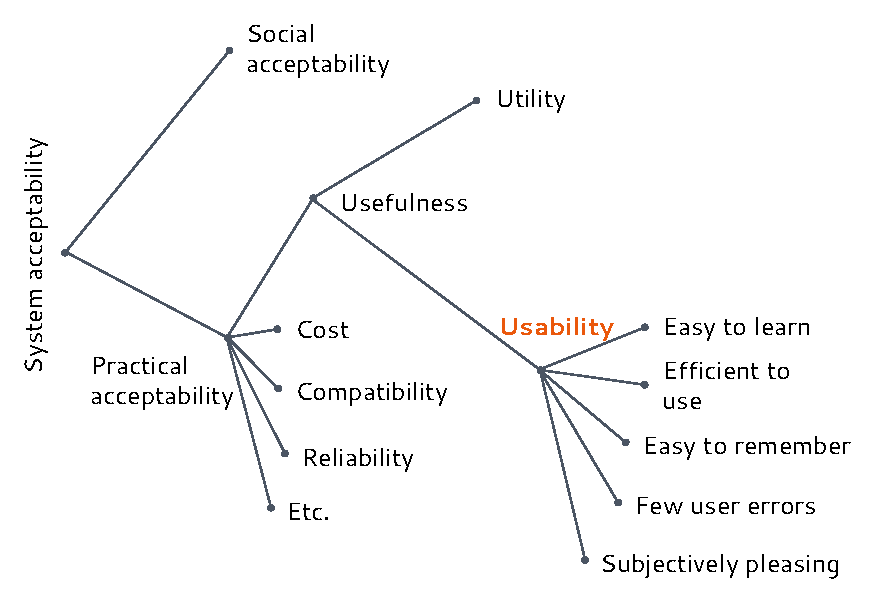
\includegraphics[height=8cm, keepaspectratio]{System_Acceptability_Map}
    \caption{Usability in the context of System Acceptability \parencite{Wilson_2009}.}
    \label{fig:system-acceptability}
\end{figure}

The \gls{cue} model introduced by \textcite{Thüring_Mahlke_2007} discerns between "instrumental" and "non-instrumental" qualities \parencite[p. 1209]{Juergen_et_all_2020}.
Similarly, \textcite{Hassenzahl_2008} distinguish between "pragmatic" and "hedonic" qualities \parencite[p. 1209]{Juergen_et_all_2020}.
Both former categories match the first four qualities mentioned by \textcite{Nielsen_1993}, while the latter are closer to Satisfaction and encompass, e.g., visual aesthetic, relatedness, or stimulation \parencite{Thüring_Mahlke_2007, Hassenzahl_2008}.

\subsection{Evaluation}
\label{Literature-HSIE-Evaluation}

\subsubsection{Accessibility}

\textcite{WAI_Evaluation} acknowledges two ways to evaluate the Accessibility of web services akin to the two kinds of Accessibility requirements outlined in \ref{Kinds-of-Accessibility}:

\begin{itemize}
    \item using tools - software can automatically check a service against standards like \gls{wcag} or assist humans but cannot solely determine whether a web service is Accessible \parencite{WAI_Evaluation_Tools},
    \item with the assistance of humans as target users - users without disabilities or with different disabilities can be involved in evaluating Accessibility but alone cannot determine whether a web service is Accessible \parencite{WAI_Evaluation_Users}.
\end{itemize}

A comprehensive evaluation of conformance to \gls{wcag} can be performed using \gls{wcagem} \parencite{WAI_Evaluation_Methodology}.
It can be used for self-assessment or assessment by a third party and can involve both tools and users \parencite{WAI_Evaluation_Methodology}.
\textcite{WAI_Evaluation_Methodology} provides the five steps that make up the \gls{wcagem}, and that can be executed with the help of \gls{wcagem} Report Tool\footnote{\gls{wcagem} Report Tool is available online at \url{https://www.w3.org/WAI/eval/report-tool}.}:

\begin{enumerate}
    \item Determine the overall scope - define the evaluated subject, baseline, and objectives, including the mentioned \gls{wcag} version and conformance level - A, AA, or AAA - with AAA being the strictest one and AA being the recommended one.
    \item Explore the subject - find what are the used technologies, e.g., HTML, WAI-ARIA, or MathML, and identify essential functionality or types of content, e.g., authentication, check-out, or blog pages.
    \item Pick sample from the subject - pick specific (random) \glspl{url} representative of the findings from the previous step or all available \glspl{url} if possible.
    \item Evaluate the sample - follow the \gls{wcag} to gather information about compliance with all of the requirements of the relevant conformance level for each identified \gls{url}.
    \item Report the results - create a report, e.g. using the provided template, that includes an executive summary, background, scope, details about the person evaluating, review process approach and goal, and results and recommendations \parencite{WAI_Evalutation_Report}.
\end{enumerate}

\begin{figure}[H]
    \centering
    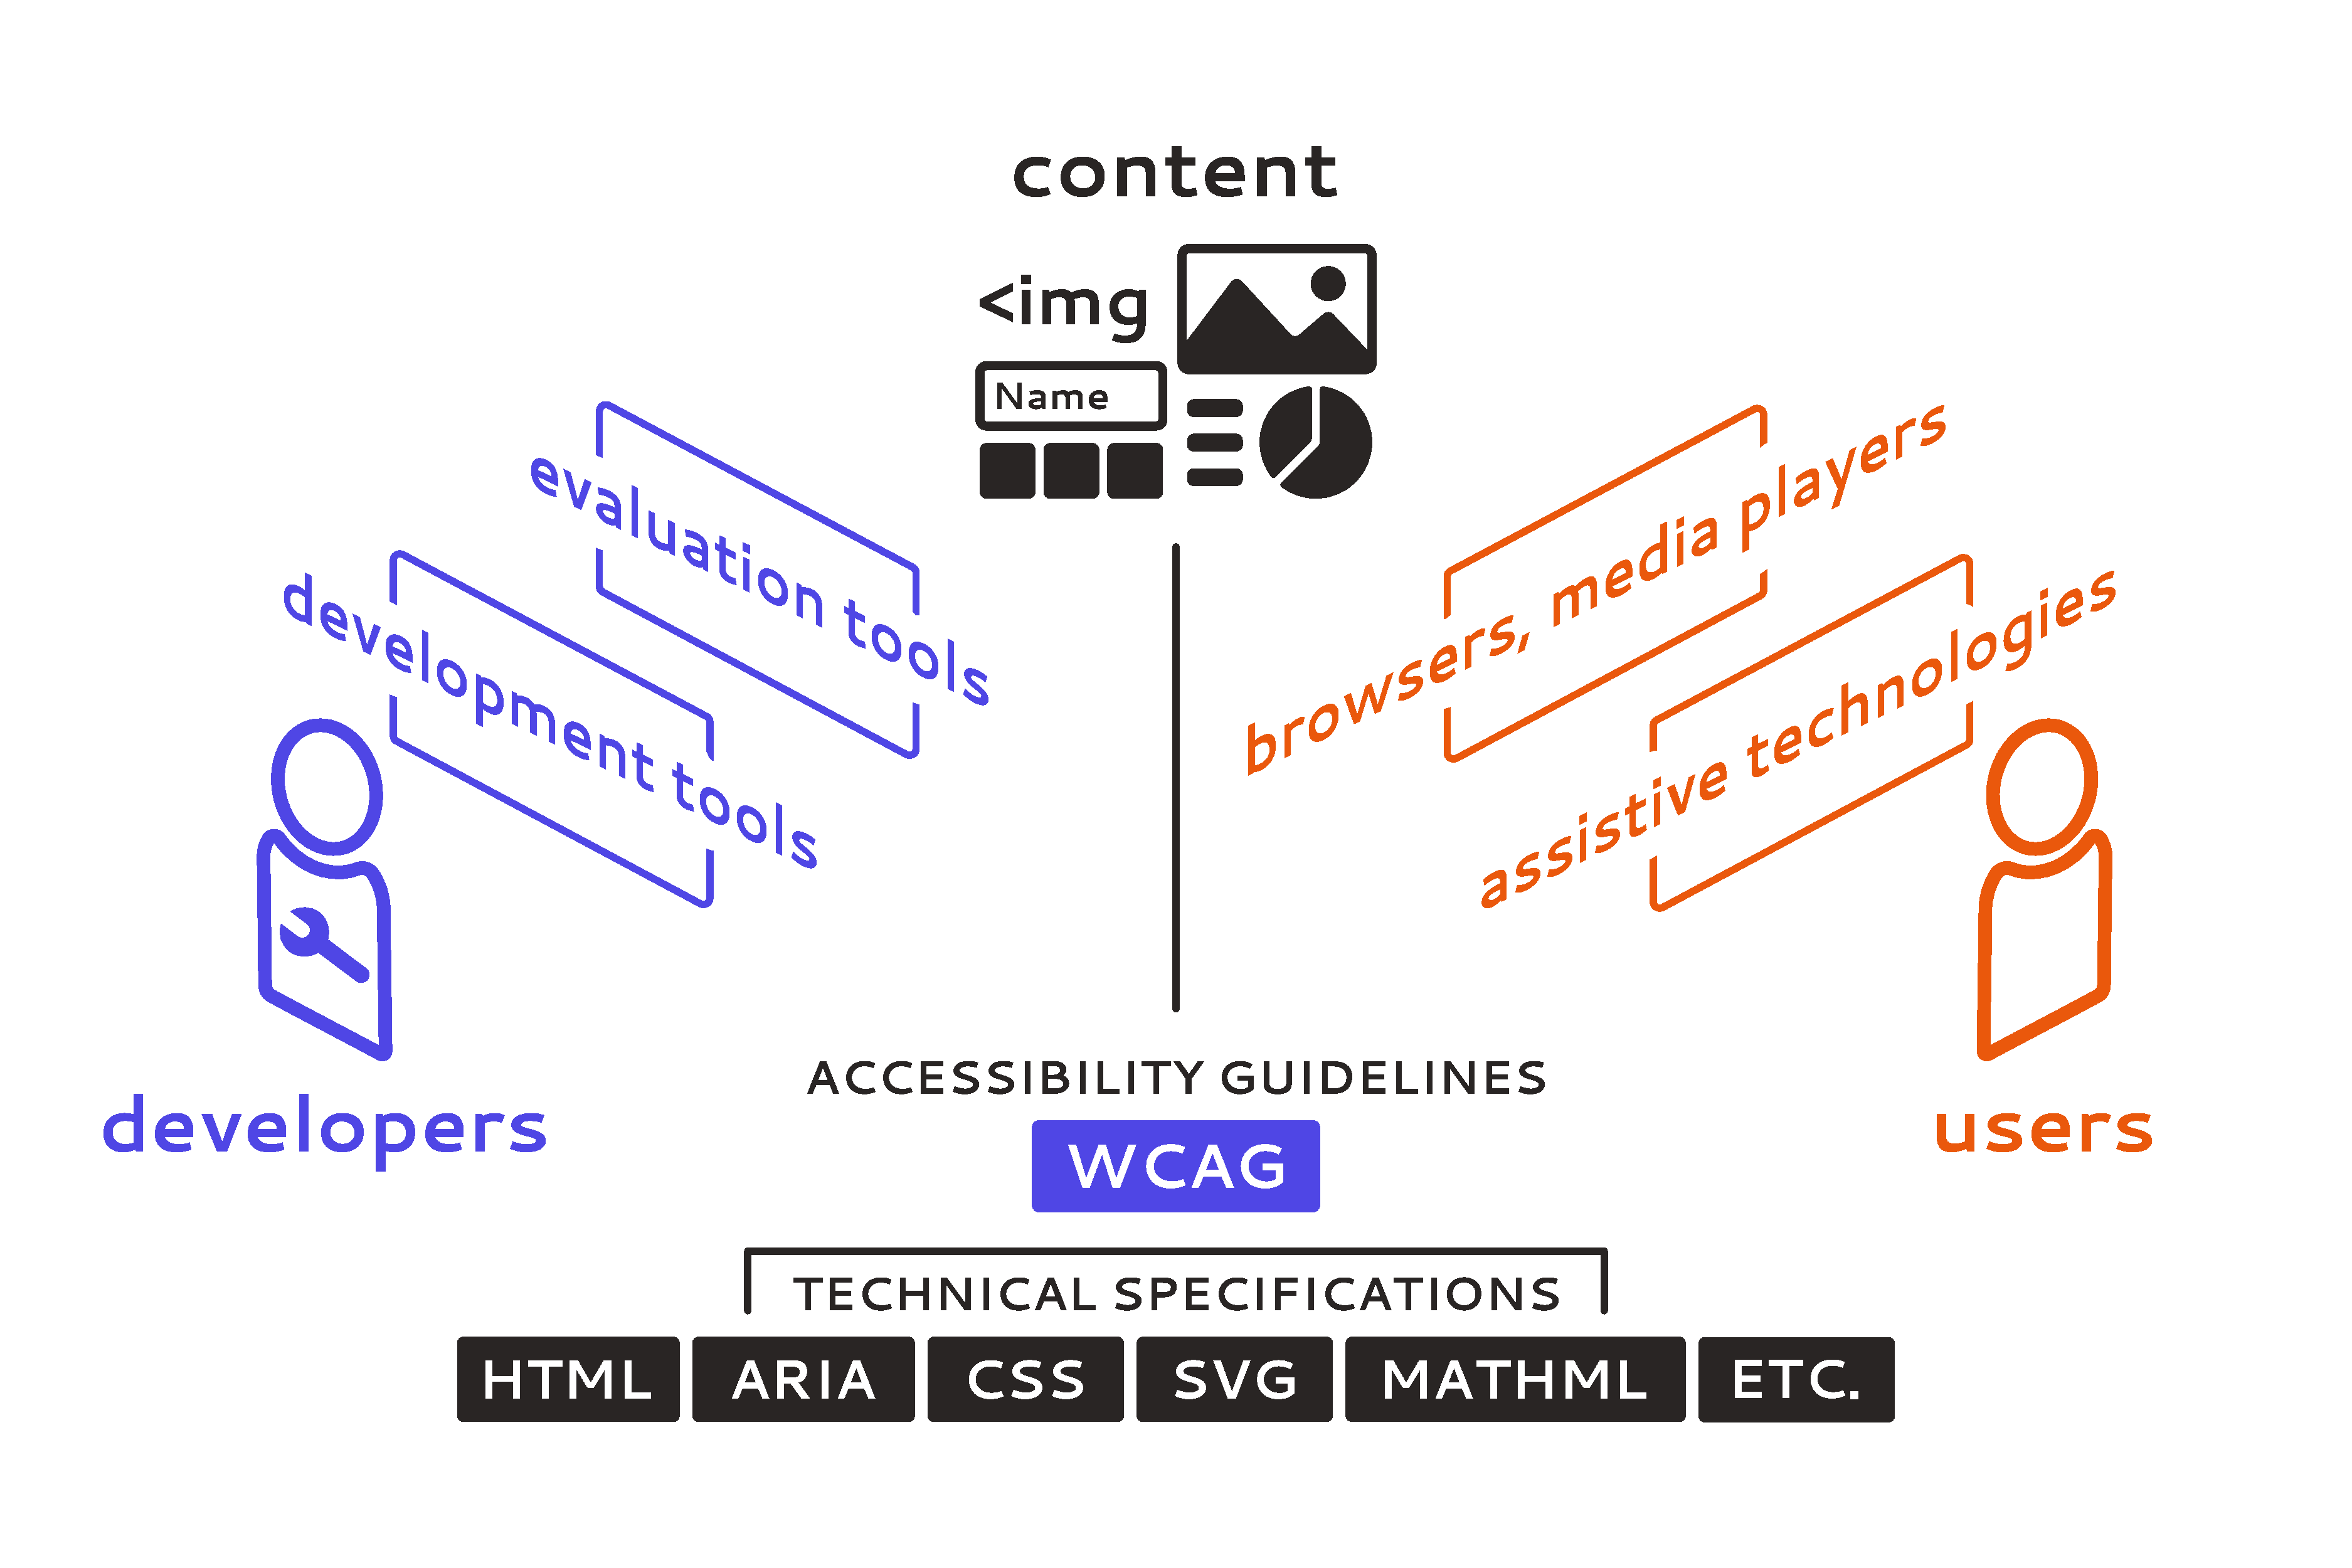
\includegraphics[height=8cm, keepaspectratio]{Accessibility_Overview_Diagram}
    \caption{Web content relation to Accessibility guidelines, users, and developers \parencite{WAI_WCAG}.}
    \label{fig:wcag-context}
\end{figure}

\label{Accessibility-Tools}

\textcite{WAI_Evaluation_Tools} mentions a wide variety of (semi) automated evaluation tools are available to cover different guidelines, languages, or technologies and working with different environments, inputs, and outputs.
Three examples of types of tools in regards to the mode of operation include \glspl{api}, browser plugins, and online services\footnote{A list of web accessibility evaluation tools maintained by \gls{wai} is available online at \url{https://www.w3.org/WAI/ER/tools}.} \parencite{WAI_Evaluation_Tools}.
Findings from \textcite{Frazão_Duarte_2020}, who reviewed the currently available most popular browser plugins, support the recommendation from \gls{wai} on the need to use multiple tools and the need to perform manual actions on top of the automated checks.
For example, the most popular one, Google's Lighthouse, based on the aXe engine, checks for 19 criteria compared to TotalValidator's 50, and it seems to be more efficient in one kind of criteria while the others are more efficient at finding errors relevant for other criteria \parencite{Frazão_Duarte_2020}.
As far as evaluation with the assistance of users is concerned, \textcite{WAI_Evaluation_Users} warns users having different backgrounds and representing different groups should be ideally involved to capture a wide variety of real potential users and to eliminate subjectivity.
\textcite{Wegge_Zimmermann_2007} reiterate Accessibility evaluation involves users from different groups that can tell whether the service can be used with their disability, is compatible with their assistive technology, or if the service behaves the way they expect.

\subsubsection{Usability and \gls{ux}}

\textcite{Wegge_Zimmermann_2007} mention that Usability, in contrast to Accessibility, is not typically tested by adherence to standards but by testing and analysing the impact on the end-users.
\textcite{Edyburn_2021} adds that we can monitor subjective measures like decreased frustration or objective measures like increased productivity.

A distinction is pointed to by \textcite{Juergen_et_all_2020}, who reiterate two kinds of Usability testing:

\begin{itemize}
    \item formative - helps pinpoint and solve problems with service during the development - called "diagnostic usability" by \textcite{Lewis_2014},
    \item summative - evaluates a service to compare it to other service or criteria - called "measurement-based usability" and told to have similarities to experimental psychology by \textcite{Lewis_2014}.
\end{itemize}

\textcite{Juergen_et_all_2020} also argue that the same thinking could be followed when evaluating \gls{ux} as well, even though such explicit distinction has not been made yet in regards to \gls{ux}.
There is a large number of concrete methods that could be utilised, like questionnaires, observation, interviews, data logging, or user testing \parencite{Juergen_et_all_2020}.
While expert-based methods are seen as more cost-effective, some argue they do not reflect real use the way user-based do, and user-based methods can generate a broader range of data \parencite{Juergen_et_all_2020}.
\textcite{Juergen_et_all_2020} argue a "principal method" to evaluate the Usability of a service is user testing - users use artefact watched by observers that acquire objective quantitative data, e.g., on efficiency or errors.
All while focusing on specific roles and tasks \parencite{Wegge_Zimmermann_2007,McCloskey_2014}.

\gls{ux} evaluation that takes into consideration emotion (i.e. not or not only Usability) is argued to be harder to evaluate since it is very individual \parencite{Juergen_et_all_2020}.
Therefore, expert-based methods are replaced by user-based methods that can be based on more broad but still subjective established questionnaires like \gls{mecue} \parencite{Juergen_et_all_2020}.
Considering another angle of subjective \gls{ux} evaluation that includes Usability, \textcite{Lewis_2014} asserts practitioners should use standardised Usability questionnaires which are proven to reliably assess perceived Usability and are referenced in national and international standards.
For example, \gls{sus} \parencite{Lewis_2018} or \gls{pssuq} \parencite{Lewis_1995, Lewis_2002}.
Both of these standardised questionnaires are available for free, should produce statistically significant data, and have a relatively low number of items - 10 for \gls{sus} and 16 for \gls{pssuq} \parencite{Lewis_2014}.
An even shorter alternative that has only slightly lower reliability ($r>0.8$ compared to $r>0.9$) and seems to produce results correlated to \gls{sus} repeatedly is \gls{umux} with four items and its shorter variant \gls{umux}[-LITE] with two items \parencite{Lewis_2014,Lewis_2018}.
\textcite{Schrepp_Kollmorge_Thomaschewski_2023} suggest that based on their findings researchers can feel confident choosing \gls{sus} or \gls{umux}[-LITE] if the main objective are Usability-focused aspects.
That is mainly thanks to the focus on the Usability aspects that makes these variants lend themselves well to professional software \parencite{Schrepp_Kollmorge_Thomaschewski_2023}.
The same cannot be said about software where the software is used for leisure as \textcite{Schrepp_Kollmorge_Thomaschewski_2023} mention only questionnaires like \gls{ueq-s} were able to capture hedonic qualities.

\label{sec:sus-evaluation}

Some questionnaires like the mentioned \gls{sus} have a long history and so can offer useful suggestions based on the data from years of use \parencite{brooke_2013}.
For example, \textcite[p. 35]{brooke_2013} points out that the word "cumbersome" used in one of the questions is not easily understood by non-native English speakers.
To address this problem, \textcite[p. 35]{brooke_2013} suggests it can be replaced with the word "awkward", citing several supporting studies.
In terms of interpreting the resulting \gls{sus} score, \textcite[pp. 36-37]{brooke_2013} points out there are data-backed ways to assign a grade and an adjective to resulting scores the way \textcite{bangor_determining_2009} and \textcite{sauro_practical_2011} did.

In relation to e-learning software, in particular, \textcite{Darin_et_all_2019} also mention that commonly used instruments are questionnaires.
That being said, \textcite[p. 60]{Darin_et_all_2019} also point to "a rising trend [of capturing both] self-reported data [and] UX measurement, in quali-quantitative approaches".
A more specific and objective alternative to capturing emotional aspects can be physiological data like body posture \parencite{Tan_Schöning_Luyten_Coninx_2013}.
However, these can come with privacy challenges and difficulties evaluating the data \parencite{Juergen_et_all_2020}.

In regards to the design of Usability testing, \textcite{McCloskey_2014} mentions that user tasks should capture key user goals, prompt users to take action, and be engaging by providing context without giving out any clues.
Remote Usability testing can, but does not have to, involve interactive sessions between user and facilitator and can be done using automated tools \parencite{Moran_2019}.
Formative Usability testing is likely to be qualitative, and even several users can identify most of the problems \parencite{Lewis_2014,Moran_2019}.
On the other hand, summative Usability testing is more likely to be quantitative and can be used to compare \parencite{Macefield_2009, Moran_2019}.

Some of the most common quantitative metrics are task success rate and time on task \parencite{Macefield_2009, Moran_2019}.
\textcite{Macefield_2009} mentions that these are suitable for analysis using statistical methods and can be used to make important decisions like go/no-go for new systems.
When processing time on task data, \textcite{sauro_chapter3_2016} suggest using geometric mean, rather than mean or median, as it seems to have a considerably lower error and bias on smaller sample sizes ($n < 25$).
However, when comparing two systems, \textcite{sauro_chapter5_2016} do not think it is worth it to use geometric mean as "two-tailed paired $t$-test is widely considered robust to violations of normality".

\textcite{Lewis_2014} contends there is no universal number of participants for summative studies, and one should try to utilise available tools to calculate the required number of participants.
\textcite{Macefield_2009} mentions that a comparative study is essentially a hypothesis test where the aim is to collect evidence a software A has better Usability metrics than software B.
As such, it is important to ensure the results are statistically significant by having a low probability ($p \leq 0.1 $, ideally $p \leq 0.05 $) of the \textit{null hypothesis} \parencite{Macefield_2009}.
Since increasing the number of participants should lower this probability, \textcite{Macefield_2009} suggests one can run the study until statistical significance is reached or the test fails.
Based on the previous data across the field, \textcite{Macefield_2009} hints that a study group should not be smaller than eight participants, with ten to twelve participants being likely to result in statistically significant data.
The same suggestion seems to apply specifically to questionnaires examining Usability on the web as well, with \gls{sus} achieving the "correct" conclusion 100\% of the time with twelve and more participants on data with a large effect size \parencite{tullis_comparison_2004}.
The relation between the sample size and the probability a "correct" conclusion is reached involving different questionnaires can be seen in Figure~\ref{fig:hsie-questionnaire-sample-size}.

\begin{figure}[H]
    \centering
    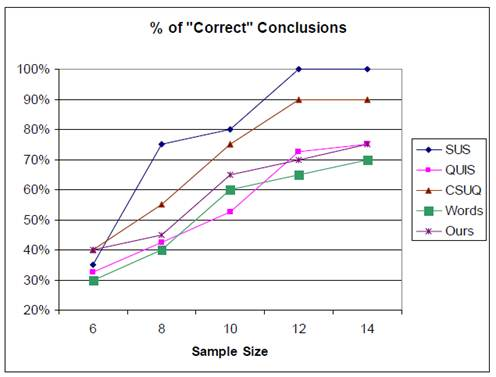
\includegraphics[height=8cm, keepaspectratio]{Sample_Size_Correct}
    \caption{Sample size vs "correct" conclusions \parencite{tullis_comparison_2004}.}
    \label{fig:hsie-questionnaire-sample-size}
\end{figure}

\textcite{Macefield_2009} mentions that the size of the effect has a strong influence on the required number of participants, and \textit{power analysis} can be done at different stages to verify the sample size required for statistically significant data or significance in general.
However, \textcite{Dziak_Dierker_Abar_2020} argue that using power analysis to decide significance during or after the study (post hoc) should never be done.
Alternatives suggested by \textcite{Dziak_Dierker_Abar_2020} for this purpose are \textit{confidence intervals} and \textit{Bayesian analysis}.
That being said, \textcite{Dziak_Dierker_Abar_2020} admits Bayesian analysis is not yet very commonly understood.
\textcite{sauro_chapter5_2016} concur with the use of confidence invervals when comparing \gls{sus} scores or time on task times.
If a between-subjects comparison is performed, \textcite{sauro_chapter5_2016} suggest the use of two-sample $t$-test to take into consideration both variation within the group and between the groups.
The relevant formula can be seen in Figure~\ref{fig:hsie-two-sample-t-test}, where $\hat{x}_1$ and $\hat{x}_2$ are means of data for system 1 and 2, $s_1$ and $s_2$ are respective standard deviations, and $n_1$ and $n_2$ are respective sample sizes.

\begin{figure}[H]
    \[ t = \displaystyle\frac{\hat{x}_1-\hat{x}_2}{\displaystyle\sqrt{\frac{s^2_1}{n_1}+\frac{s^2_2}{n_2}}} \]
    \caption{Two-sample $t$-test formula \parencite{sauro_chapter5_2016}.}
    \label{fig:hsie-two-sample-t-test}
\end{figure}

The confidence interval can then be calculated using formula in Figure~\ref{fig:hsie-confidence-interval-diff}, where $t_a$ is "the critical value from the $t$-distribution for the specified level of confidence and degrees of freedom" \parencite{sauro_chapter5_2016}.

\begin{figure}[H]
    \[ (\hat{x}_1-\hat{x}_2) \pm t_a\displaystyle\sqrt{\frac{s^2_1}{n_1}+\frac{s^2_2}{n_2}} \]
    \caption{Confidence interval formula \parencite{sauro_chapter5_2016}.}
    \label{fig:hsie-confidence-interval-diff}
\end{figure}
